\documentclass[10pt]{article}
\usepackage{graphicx}
\usepackage[margin=1.5cm]{geometry}
\usepackage{amsmath}
\def\brcurs{{\mbox{$\resizebox{.16in}{.08in}{
\includegraphics{BoldR}}$}}}
\def\rcurs{{\mbox{$\resizebox{.16in}{.08in}{
\includegraphics{ScriptR}}$}}}

\begin{document}
\twocolumn

\title{Thursday Warm-up: Potentials}
\author{Prof. Jordan C. Hanson}

\maketitle

\section{Memory Bank}

\small

\begin{itemize}
\item \textbf{Gradient} in spherical coordinates:
\begin{equation}
\nabla V = \frac{\partial V}{\partial r}\hat{\mathbf{r}}+\frac{1}{r}\frac{\partial V}{\partial \theta}\hat{\boldsymbol{\theta}} + \frac{1}{r\sin\theta}\frac{\partial V}{\partial \phi}\hat{\boldsymbol{\phi}}
\end{equation}
\item \textbf{Laplace's equation} in spherical coordinates, with azimuthal symmetry:
\begin{equation}
\frac{\partial}{\partial r}\left(r^2\frac{\partial V}{\partial r}\right) + \frac{1}{\sin\theta}\frac{\partial}{\partial \theta}\left(\sin\theta \frac{\partial V}{\partial \theta}\right) = 0
\end{equation}
\item \textbf{Multipole expansion} in spherical coordinates:
\begin{equation}
V(r,\theta) = \frac{1}{4\pi\epsilon_0}\sum_{n = 0}^{\infty} \frac{1}{r^{n+1}} \int (r')^n P_n(\cos\alpha)\rho(\mathbf{r}') d\tau' \label{eq:mult}
\end{equation}
\end{itemize}

\begin{figure}
\centering
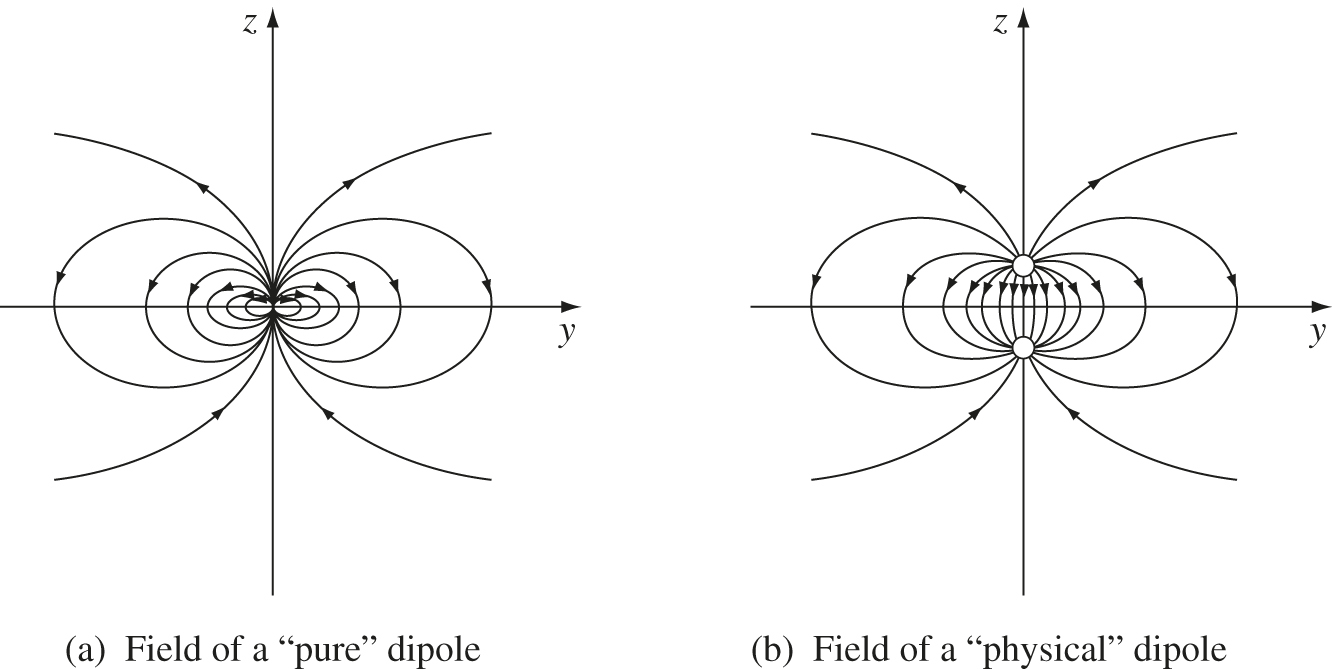
\includegraphics[width=0.49\textwidth,trim=0cm 1cm 0cm 0cm,clip=true]{figures/3_37.jpg}
\caption{\label{fig:1} (Left) A dipole in the limit that $d\to 0$ and $q\to\infty$. (Right) A physical dipole.}
\end{figure}

\section{Multipole Expansion}

\begin{enumerate}
\item Generate the approximate voltage of a physical dipole aligned with the z-axis ($n=1$ in Eq. \ref{eq:mult}, and $P_1(x) = x$).  \\ \vspace{3.5cm}
\item In analogy to the \textit{moment} of a probability distribution function (PDF) let the \textbf{dipole moment} of a charge distribution be
\begin{equation}
\mathbf{p} = \int \mathbf{r}' \rho(\mathbf{r}') d\tau'
\end{equation}
Show that the dipole moment is independent of a shift in the origin, if the total charge is zero. \\ \vspace{3.5cm}
\item Formulate the expression for the voltage of the dipole in terms of the dipole moment.  Note that $\hat{\mathbf{r}} \cdot \mathbf{r}' = \cos\theta$ if $\mathbf{p}$ is along the z-axis. \\ \vspace{3.5cm}
\item Now compute the $\mathbf{E}$-field of a dipole using the gradient in spherical coordinates. \\ \vspace{3.5cm}
\item List the magnitude and direction of the $\mathbf{E}$-field at the following points:
\begin{itemize}
\item A point far from the origin, on the xy-plane.
\item A point far from the origin, on the z-axis.
\item A point far from the origin, on the -z-axis.
\end{itemize} \vspace{2cm}
\item \textbf{Think conceptually.} What is the sum of the monopole and dipole terms in the multipole expansion for a charge distribution comprized of two anti-parallel dipoles?
\end{enumerate}

\end{document}
